\section{Disjoint Set Union on Tree}

\begin{frame}
\frametitle{Disjoint Set Union on Tree}
We have to maintain the original tree to preserve the ability to rollback the connection.

\medskip

Let's recall the original parent array definition.

\begin{block}{Definition: Parent Array}
    parent[u] := direct parent of vertex $u$ but if $u$ has no parent parent[u] will store itself.
\end{block}

But... we have to change \textcolor{blue}{how we unite the sets}.

\end{frame}

\begin{frame}
\frametitle{Disjoint Set Union on Tree}
There are two main approaches to uniting in the disjoint set union on a tree:

\begin{itemize}
    \item Union by Rank
    \item Union by Size
\end{itemize}

\begin{block}{Definition: Rank}
     In this scope, rank is used to represent the height (or depth) of the tree.
\end{block}

But these two approaches use the same main idea, which is ``merge small to large".

\end{frame}

\begin{frame}[fragile]
\frametitle{Disjoint Set Union on Tree}
And we can recall the old ``find\_root" function, too.

\begin{lstlisting}[language=C++, basicstyle=\small]
int parent[N];
int find_root(int u) {
    while(u != parent[u]) {
        u = parent[u];
    }
    return u;
}
\end{lstlisting}

\end{frame}

\begin{frame}
\frametitle{Disjoint Set Union on Tree}
First, let's see how ``union by rank" works.

\begin{center}
\begin{tikzpicture}
[  
    level 1/.style={sibling distance=25mm},
    level 2/.style={sibling distance=15mm},
    edge from parent/.style={thick}
]
    \begin{scope}[edge from parent/.style={draw=red}]
        \node [draw, circle, red] {1}
            child {node [draw, circle, red] {3}}
            child {
                node [draw, circle, red] {2}
                child {node [draw, circle, red] {4}}
            };
    \end{scope}
    
    \begin{scope}[edge from parent/.style={draw=orange}]
        \node [draw, circle, orange] at (6,0) {5}
            child {node [draw, circle, orange] {6}};
    \end{scope}
\end{tikzpicture}
\end{center}

\end{frame}

\begin{frame}
\frametitle{Disjoint Set Union on Tree}
First, let's see how ``union by rank" works.

\begin{center}
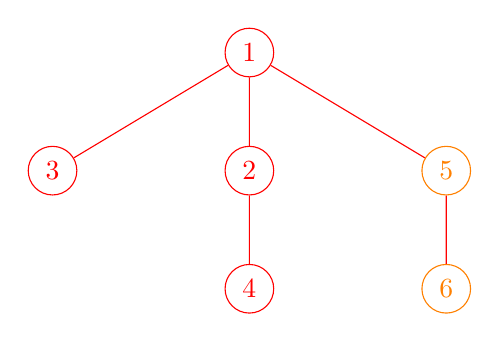
\begin{tikzpicture}
[  
    level 1/.style={sibling distance=25mm},
    level 2/.style={sibling distance=15mm},
    edge from parent/.style={thick}
]
    \begin{scope}[edge from parent/.style={draw=red}]
        \node [draw, circle, red] {1}
            child {node [draw, circle, red] {3}}
            child {
                node [draw, circle, red] {2}
                child {node [draw, circle, red] {4}}
            }
            child {
                node [draw, circle, orange] {5}
                child {node [draw, circle, orange] {6}}
            };
    \end{scope}
\end{tikzpicture}
\end{center}

In this case (when the main tree's rank is greater than the merging tree's rank), the rank does not change.

\end{frame}

\begin{frame}
\frametitle{Disjoint Set Union on Tree}
When the main tree's rank is equals to the merging tree's rank

\begin{center}
\begin{tikzpicture}
[
    edge from parent/.style={thick}
]
    \begin{scope}[edge from parent/.style={draw=red}]
        \node [draw, circle, red] {1}
            child {node [draw, circle, red] {3}}
            child {
                node [draw, circle, red] {2}
                child {node [draw, circle, red] {4}}
            };
    \end{scope}
    
    \begin{scope}[edge from parent/.style={draw=orange}]
        \node [draw, circle, orange] at (6,0) {5}
            child {
                node [draw, circle, orange] {6}
                child {node [draw, circle, orange] {7}}
            };
    \end{scope}
\end{tikzpicture}
\end{center}
    
\end{frame}

\begin{frame}
\frametitle{Disjoint Set Union on Tree}
When the main tree's rank is equals to the merging tree's rank

\begin{center}
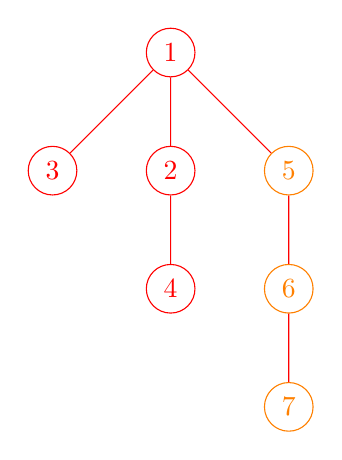
\begin{tikzpicture}
[
    edge from parent/.style={thick}
]
    \begin{scope}[edge from parent/.style={draw=red}]
        \node [draw, circle, red] {1}
            child {node [draw, circle, red] {3}}
            child {
                node [draw, circle, red] {2}
                child {node [draw, circle, red] {4}}
            }
            child {
                node [draw, circle, orange] {5}
                child {
                    node [draw, circle, orange] {6}
                    child {node [draw, circle, orange] {7}}
                }
            };
    \end{scope}
\end{tikzpicture}
\end{center}

Rank is increase by one.
    
\end{frame}

\begin{frame}[fragile]
\frametitle{Disjoint Set Union on Tree}

From observation:

\[
    \mathrm{rank}_{\mathrm{new}} = \max\{\mathrm{rank}_{\mathrm{main}}, \mathrm{rank}_{\mathrm{merging}} + 1\}
\]

\begin{lstlisting}[language=C++, basicstyle=\small]
void unite(int u, int v) {
    int ru = find_root(u), rv = find_root(rv);
    if(ru == rv) return ;
    if(rank[ru] > rank[rv]) swap(ru, rv);
    rank[rv] = max(rank[rv], rank[ru] + 1);
    parent[ru] = rv;
}
\end{lstlisting}

\end{frame}

\begin{frame}
\frametitle{Disjoint Set Union on Tree}
\begin{block}{Claim}
Union by Rank takes $\mathcal{O}(log(n))$ time per query.
\end{block}
\textit{Intuition}:
By creating tree with 
\begin{itemize}
    \item rank $2$ there should be created from tree with $2$ rank $1$ trees (requires $2$ vertices)\\
    \item rank $3$ there should be created from tree with $2$ rank $2$ trees (requires $4$ vertices)\\
    \item \dots
    \item rank $n$ there should be create from tree with $2$ rank $n-1$ trees (requires $2^{n - 1}$ vertices)
\end{itemize}

We just have $n$ vertices so that the rank of merged tree will not exceed $log(n)$. So, naive union find will run in $\mathcal{O}(log(n))$.
\end{frame}

\begin{frame}
\frametitle{Disjoint Set Union on Tree}

Now, let's see how ``union by size" works.

\begin{center}
\begin{tikzpicture}
[
    edge from parent/.style={thick}
]
    \begin{scope}[edge from parent/.style={draw=red}]
        \node [draw, circle, red] {1}
            child {node [draw, circle, red] {3}}
            child {
                node [draw, circle, red] {2}
                child {node [draw, circle, red] {4}}
            };
    \end{scope}
    
    \begin{scope}[edge from parent/.style={draw=orange}]
        \node [draw, circle, orange] at (6,0) {5}
            child {
                node [draw, circle, orange] {6}
                child {node [draw, circle, orange] {7}}
            };
    \end{scope}
\end{tikzpicture}
\end{center}

Merge the tree with the smaller size into the larger one.

\end{frame}

\begin{frame}
\frametitle{Disjoint Set Union on Tree}

Now, let's see how ``union by size" works.

\begin{center}
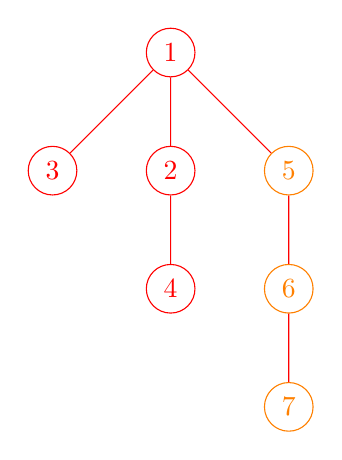
\begin{tikzpicture}
[
    edge from parent/.style={thick}
]
    \begin{scope}[edge from parent/.style={draw=red}]
        \node [draw, circle, red] {1}
            child {node [draw, circle, red] {3}}
            child {
                node [draw, circle, red] {2}
                child {node [draw, circle, red] {4}}
            }
            child {
                node [draw, circle, orange] {5}
                child {
                    node [draw, circle, orange] {6}
                    child {node [draw, circle, orange] {7}}
                }
            };
    \end{scope}
\end{tikzpicture}
\end{center}

This makes the size of tree bigger.

\end{frame}

\begin{frame}[fragile]
\frametitle{Disjoint Set Union on Tree}

\begin{lstlisting}[language=C++, basicstyle=\small]
void unite(int u, int v) {
    int ru = find_root(u), rv = find_root(rv);
    if(ru == rv) return ;
    if(sz[ru] > sz[rv]) swap(ru, rv);
    sz[rv] += sz[ru]
    parent[ru] = rv;
}
\end{lstlisting}

\end{frame}

\begin{frame}
\frametitle{Disjoint Set Union on Tree}
\begin{block}{Claim}
Union by Size takes $\mathcal{O}(log(n))$ time per query.
\end{block}
\textit{Intuition}: 
We can prove that each time merging by size

\[
    \mathrm{rank_{u}} = \log(n)
\]

where $n$ is the size of subtree of $u$

\textit{The rest is union by rank}
\end{frame}